% !Mode:: "TeX:UTF-8"
\mychapter{复杂环境下的高效自适应二维码编解码}
\label{cha:dev}

在本项目中,受制于系统的硬件规格,以及系统架构的设计要求两台设备之间完全没有物理连接以及双向通信可能,要求系统在非同步情况下对快速刷新的彩色二维码进行高速可靠的识别。由于光学信道特性以及高帧率要求较短曝光时间,摄像头拍摄到的图像会有一系列的干扰因素,使得无法获得原始编码的图像,包括线性与非线性的点位偏移,亮度、色相与饱和度的变化,色块的实际呈色与周边像素相关,直接按ISO规定算法进行解码的极高错误率使得传输实际无法进行。鉴于此,本文提出了一种复杂环境下的高效自适应二维码编解码方法,以更好的适应项目的工况。

\section{二维码重定义}

二维码本身具有容错特性。在L级别的纠错下,有约7\%的容量用于纠错;在H级别纠错下会有30\%的数据用于纠错。这使得二维码本拥有30\%的数据恢复能力。二维码的容错是由“码字”定义的,码字的具体排布如下图所示:

\begin{figure}[!htbp]
\centering
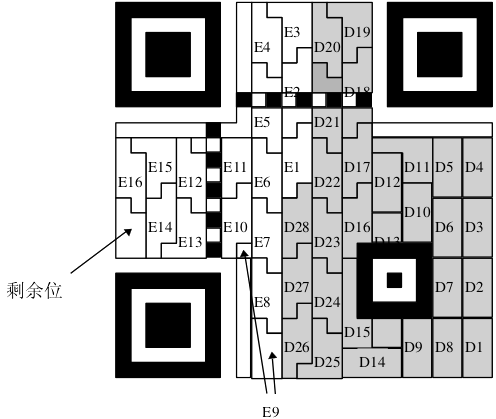
\includegraphics[scale=0.6]{figures/QR_Word.png}
\caption{二维码码字排布}
\end{figure}

QR码支持编码纯数字、数字与字符混合编码、8位字节码和包含汉字在内的多字节字符编码。除了8位字节码无压缩直接保存,其余内容都会进行压缩以增加存储容量。为保证传输的高效性,在本系统中,由于传输内容是比特流,不存在多字节字符的中国汉字与日本汉字内容,因而编码侧不会进行多字节字符的编码,解码侧也无需进行多字节字符的解码。如果使用多字节压缩,系统会因为字库原因产生数据丢失。

在国际标准二维码(以下简称ISO二维码)中,每一个码字都可以存放不同编码的内容,而二维码的容错也是由码字作为定义标准的。也就是“H级别容错最多可以允许30\%的码字发生错误”而不是“H级别容错最多可以允许30\%的码元发生错误”。在本项目的应用场景中,鉴于传输的均是8bit字节数据,并且传输的错误会随机的散步在整个二维码中,导致了30\%的码字错误率落实到码元上只能容许10\%左右的错误,在极端情况下,5\%的码元错误率会引起80\%的码字都发生错误,这是不可被接受的。因此,在编码模块中我们修改了纠错部分的定义,去除了码字概念,直接在原始的二进制数据上使用ISO二维码相同的里德-所罗门算法对信息进行编码,使得系统的可靠性有了较大的提升。

删除ISO二维码所定义的码字概念,在原始的写入数据上直接进行基于GF8的里德所罗门纠错,将纠错的数据追加到原始数据尾部。随后依照ISO/IEC 15415:2011规定的二维码写入方式,将编码后的数据写入到二维码中,可以使得二维码的纠错摆脱码字限制,回到初始的码元定义,更加符合本项目的工况。

\section{图像二值化与平滑边缘}

为了准确的获得二维码解码所需的格点信息,需要将二维码进行二值化处理以便于算法进行突变边缘的判断。

由于摄像头不可避免的存在无法即时消除的暗角,全图的亮度并不统一,没有单一的硬阈值可以使二值化有良好的效果。在正常情况下,背景和二维码目标的区分是明显的,照度是均匀的,只需要简单地使用全局二值化方法即可,常见的方法有固定阈值法、大津法、直方图双模阈值法等。在光照不均匀的情况下,这一点并不适用,固定阈值会导致全局亮度不平衡,无法正确解码,所以需要采用自适应局部阈值法来处理。

局部自适应阈值法根据每一个像素的邻域的像素值分布来确定该位置像素的二值化阈值。这样做的好处是每个像素位置的二值化阈值不是固定的,而是由周围区域的像素分布决定。一个像素的邻域如果亮度较高,那么它会被赋予较高的二值化阈值,而亮度较低的图像区域则会被赋予较小的二值化阈值。这样做可以能使得亮度不均匀的图像可以以一种较低成本的方式获得较好的二值化结果。本项目采用局部邻域块的算数平均值作为局部二值化的阈值,在有较好的效果的情况下所花时间较短。

采用局部自适应二值化,为每一个区块赋予不同的阈值,以求达到较好的二值化效果。二值化后每个像素点的值参考预期自身最近邻的k个像素点的平均亮度得到。具体可参考下式:

$$
lum_{i,j}=0.299pix_{i,j}[0]+0.587pix_{i,j}[1]+0.114pix_{i,j}[2] \geq \sum_{i-c}^{i+c}L(pix_{i,j})\quad?\quad 255\quad : \quad 0
$$

在实际应用中,对于每一个像素点都进行如上式的运算所需的时间成本是不可接受的,因此在实际应用中,采用了分块阈值的方法,将原始图像分为了一系列的网格区域,对每个区域计算平均明度,并对网格内部赋予该值作为二值化阈值。

对于二值化之后的二维码,采用了快速滑动窗口滤波,消除了局部的毛刺,为后续的检测识别流程提供了基础。快速滑动窗的实现参考下式:

$$
lum_{i,j}= (pix_{i,j} == pix_{i-1,j}\quad \&\quad pix_{i,j} == pix_{i+1,j})\quad?\quad 255\quad : \quad 0
$$
$$
lum_{i,j}= (pix_{i,j} == pix_{i,j-1}\quad \&\quad pix_{i,j} == pix_{i,j+1})\quad?\quad 255\quad : \quad 0
$$

\section{二维码格点识别}

由二维码的寻像图形与校正符推理得到二维码数据块之间的偏移量(一阶差分)与偏移量变化(二阶差分),线性偏移即可得出只发生梯度变化时每个模块的位置。

由于摄像头与屏幕之间的位置限制,必须采用球面镜头进行拍摄,使得最终得到的画面会发生鱼眼形变。在项目中,尝试过基于摄像机与镜头内参的鱼眼矫正方法,但效果不能令人满意。摩尔纹也对项目造成了影响\cite{zhang2022mobiscan}。原始图片以及基于线性推移算法得到的结果如图3.2与图3.3所示。

\begin{figure}[!htbp]
\centering
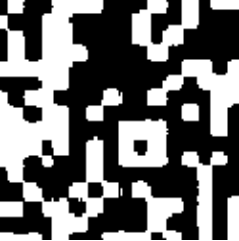
\includegraphics[scale=1]{figures/QR_Cap_00.png}
\caption{二值化后的二维码}
\end{figure}
\begin{figure}[!htbp]
\centering
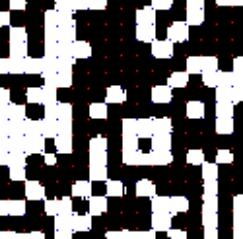
\includegraphics[scale=1]{figures/QR_Cap_GF.png}
\caption{错误的格点识别结果}
\end{figure}

不难看出,算法返回的格点中心位置与实际的格点中心位置存在一定偏移。这会对后续的解码算法造成非常显著的影响,因为格点识别的准确率会直接影响最终的信息解码率。为了解决线性变化与非线性变化,在固定二阶差分偏移的基础上,每一个生成的点需要主动的感知其在空间中的位置,及时的对二阶差分产生的误差进行矫正。为此,项目实现了一套基于专家系统的自感知格点校正系统。具体流程由下例以及图3.4到图3.13阐释。

第一步,获取先验知识,由先前得到的点序列求出平均偏移向量。

\begin{figure}[!htbp]
\centering
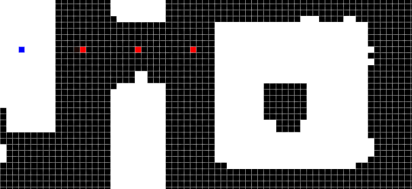
\includegraphics[scale=1]{figures/QR_Prf/图片1.png}
\caption{步骤一}
\end{figure}

第二步,根据先验知识,线性推算下一个点的坐标。

\begin{figure}[!htbp]
\centering
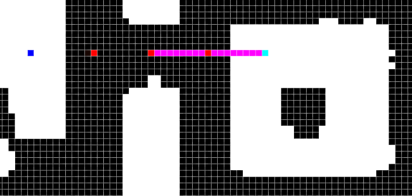
\includegraphics[scale=1]{figures/QR_Prf/图片2.png}
\caption{步骤二}
\end{figure}

第三步,确定扫描方向,在最边缘一圈的点无需进行某些方向的扫描,因为不会得到结果。由于这一点为图像中任意一点,故需要进行四个方向的探测。

\begin{figure}[!htbp]
\centering
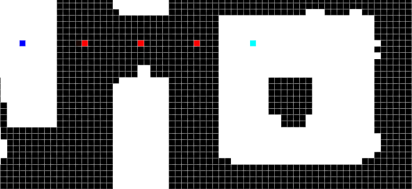
\includegraphics[scale=1]{figures/QR_Prf/图片3.png}
\caption{步骤三}
\end{figure}

第四步,向上探测,获取最近邻突变点坐标。

\begin{figure}[!htbp]
\centering
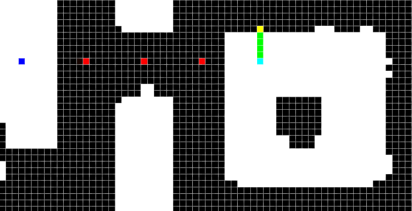
\includegraphics[scale=1]{figures/QR_Prf/图片4.png}
\caption{步骤四}
\end{figure}

第五步,向下探测,获取最近邻突变点坐标。

\begin{figure}[!htbp]
\centering
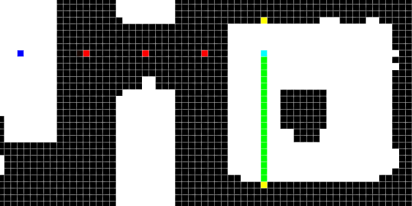
\includegraphics[scale=1]{figures/QR_Prf/图片5.png}
\caption{步骤五}
\end{figure}

第六步,依据上下突变点坐标、距离,参考先验的平均偏移向量,重新计算自身的y轴坐标。

\begin{figure}[!htbp]
\centering
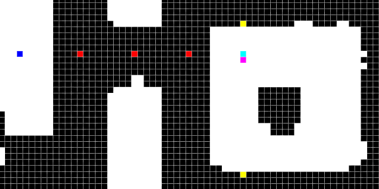
\includegraphics[scale=1]{figures/QR_Prf/图片6.png}
\caption{步骤六}
\end{figure}

第七步,移动扫描起点。

\begin{figure}[!htbp]
\centering
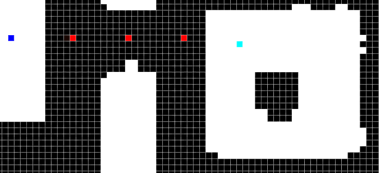
\includegraphics[scale=1]{figures/QR_Prf/图片7.png}
\caption{步骤七}
\end{figure}

第八步,向左探测,获取最近邻突变点坐标。

\begin{figure}[!htbp]
\centering
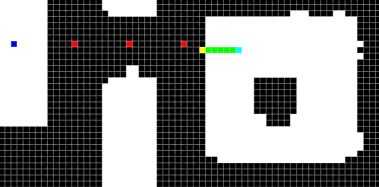
\includegraphics[scale=1]{figures/QR_Prf/图片8.png}
\caption{步骤八}
\end{figure}

第九步,向右探测,获取最近邻突变点坐标。

\begin{figure}[!htbp]
\centering
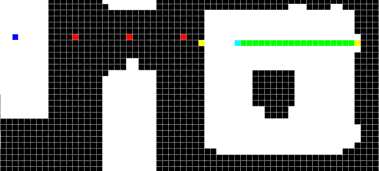
\includegraphics[scale=1]{figures/QR_Prf/图片9.png}
\caption{步骤九}
\end{figure}

第十步,依据左右突变点坐标、距离,参考先验的平均偏移向量,重新计算自身的x轴坐标。

\begin{figure}[!htbp]
\centering
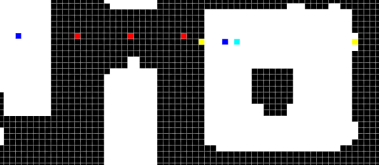
\includegraphics[scale=1]{figures/QR_Prf/图片10.png}
\caption{步骤十}
\end{figure}

由此,可以更为准确的获得自身的位置坐标。此外,基于点对之间的位置关系,可以进行基于最近n个点的移动平均校正,将少数偏移点的位置进行校正与恢复。基于专家系统的自适应格点识别算法结果如图3.14所示。

\begin{figure}[!htbp]
\centering
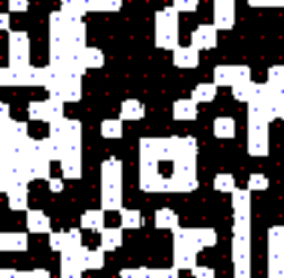
\includegraphics[scale=1]{figures/QR_Prf/图片11.png}
\caption{正确的格点识别结果}
\end{figure}

\section{基于位置缓存的二维码加速识别}

为了实现高速的二维码识别,针对二维码位置不变的特点,本项目软件部分设计了二维码位置缓存私有解码算法,可使二维码解码速率大大提升。

二维码的识别过程首先进行的是寻像图形的定位,根据辅助定位块进行偏移纠正,而后读取版本信息,根据偏移量获得每次一个二维码信息块的位置。这一过程往往通过遍历完成,在一个高分辨率的图像中进行这样的遍历过程是非常耗时的。

由于摄像头与屏幕的相对位置不发生变化,二维码在屏幕中的位置也不发生变化,因此上述的定位过程在实际执行时,每次返回的都是相同的结果。利用这一点,可以在后续的识别过程中使用之前的定位结果,跳过长耗时的处理流程,达到加速解码的目的。二维码加速识别的流程如下图所示:

\begin{figure}[!htbp]
\centering
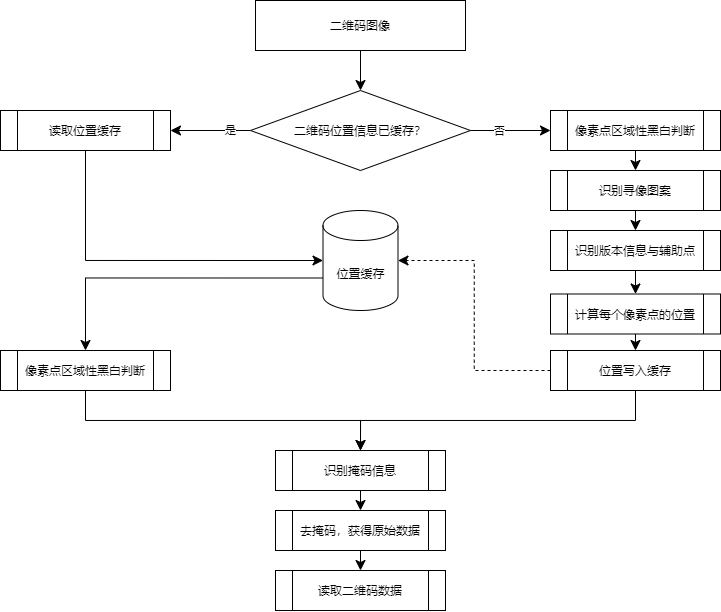
\includegraphics[scale=0.5]{figures/QR_Prf/QR_Fast.png}
\caption{二维码加速识别}
\end{figure}

为了防止错误的位置缓存对二维码的识别结果造成影响,二维码的位置缓存也有自身的刷新模式,分为定时刷新与触发刷新。在定时刷新模式下,每隔给定的Interval帧重新初始化一次格点,当Interval为0时,退化到没有位置缓存的情况。在触发刷新模式下,位置缓存会捕获自身的环境变量来尝试了解后续解码的情况,当连续Counter帧都不能成功解码时,重新初始化一次格点。

\section{基于机器学习的色彩分类}

暗角效应与色彩混叠会对颜色识别造成巨大干扰。直接采用得到的彩色图像效果会引起非常低质的解码结果。为了抵消在成像环节产生的干扰因素,需要在获取彩色图像的基础上进行包括暗部补偿(消除暗角效应)、色彩校正与白平衡的一系列图像处理操作,尽可能还原原始图像。摄像头捕获到的原始图像如下图所示。

\begin{figure}[!htbp]
\centering
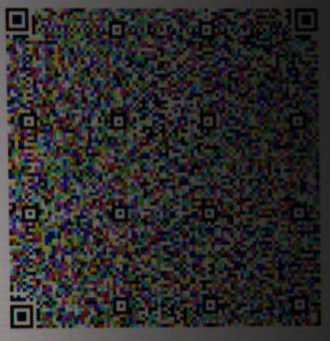
\includegraphics[scale=1]{figures/QR_Cap_RAW.png}
\caption{拍摄到的二维码图像}
\end{figure}

白平衡是一个描述屏幕中红、绿、蓝三原色混合产生的白色的准确性的指标。白平衡是一个非常重要的概念,可以用来解决一些色彩再现和色调处理问题。其基本概念是:"白色物体无论在何种光源下都能再现为白色",在某一特定光源下拍摄时发生的任何色差都可以通过放大相应的补色来进行补偿。通过白平衡补偿,我们可以在一定程度上消除画面的整体色彩偏差。\cite{陈申渭2019摄屏类图像重构算法}

暗角是由于镜头系统的光学特性而在摄影图像中观察到的径向亮度下降。在数字摄影中,相机传感器的方向性灵敏度曲线进一步增加了这种影响。在\cite{zheng2008single,lopez2015revisiting}中介绍了一种新的方法,用于对单一图像中的暗角进行免校准的追溯校正,将信息最小化的概念应用于暗角校正,使用对数强度熵作为一种具有卓越收敛特性的强度伪影校正的缩放不变量信息测量。其次,一个受限的径向多项式消隐函数确保了单调的强度曲线。由此产生的消光算法在计算上是非常高效和稳健的,基于此方法可以有效的减少暗角效应对于结果的影响。

在完成色彩的初步恢复之后,需要进行通道分离,将RGB色彩空间的图像转变为八分类或是三个二分类的一个结果,完成原始二维码数据的提取。

\begin{figure}[!htbp]
\centering
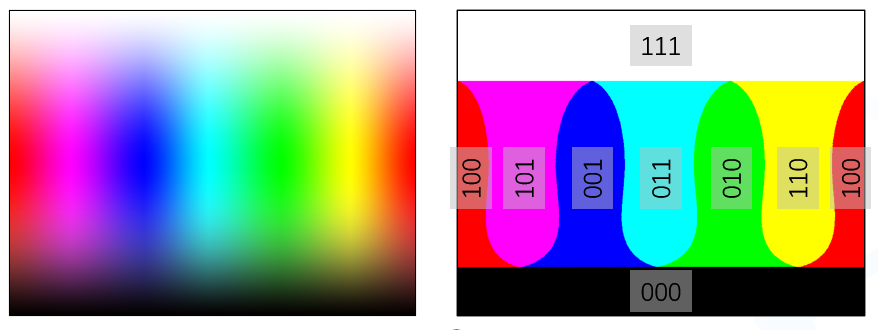
\includegraphics[scale=0.5]{figures/Color_Sp.png}
\caption{基于阈值的二维码色彩分类}
\end{figure}

基于采集得到的图片,即使是在完成了上述的各种修复流程后,也不能直接依靠阈值对色彩进行区分。在不同的图像区域,视周边颜色的不同,同一种基础色会发生较为严重的色彩偏移。加之拜耳阵列相机对于色彩混叠区域的色彩还原本身就有一定的欠缺,因此需要其他工具的引入。

\begin{figure}[!htbp]
\centering
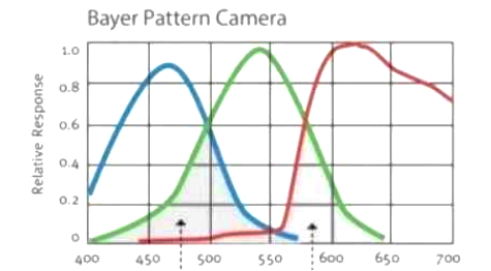
\includegraphics[scale=0.8]{figures/Color_Ba.png}
\caption{拜耳阵列相机颜色响应曲线}
\end{figure}

在本项目中,受到论文\cite{yang2018robust}的启发,使用一个SVM或逻辑斯蒂回归器进行色彩的直接8分类,利用统计学原理获得最大概率似然输出。

\begin{figure}[!htbp]
\centering
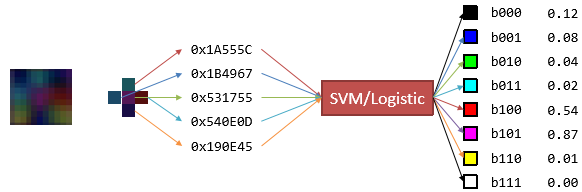
\includegraphics[scale=1]{figures/Color_Lo.png}
\caption{机器学习二维码色彩分类流程}
\end{figure}

采集了250万条清晰的数据样本,每个样本包含二维码信息块中心像素的颜色以及其最临近的8个二维码信息块中心像素的颜色,共9个RGB融合为一个27维向量作为分类器输入,8分类的置信度作为分类器输出。在构建的测试集上准确率可以达到98.6\%。在实际使用场景中,由于系统不同步带来的拍摄问题,可能会有画面刷新不完全等因素,造成准确率的下降,但总体准确率在85\%以上。

\section{基于二维码的数据传输协议MTPOQ}

MTPOQ(Message Transmission Protocol Over QR-Code,基于二维码的信息传输协议)是本项目设计中为了完成数据在二维码信道上进行无差错传输而设计的专用私有数据传输协议。

\begin{table}[htb]
  \centering
  \begin{minipage}[t]{0.8\linewidth} 
  \caption[MTPOQ组成]{MTPOQ组成}
  \label{tab:template-files}
    \begin{tabularx}{\linewidth}{lX}
      \toprule[1.5pt]
      {\heiti 字段名} & {\heiti 描述} \\\midrule[1pt]
      SN    & [2Byte] 任务序列号 \\
      PN    & [2Byte] 分包偏移量 \\
      TP    & [2Byte] 总发包数量 \\
      Data  & [不超过二维码上限] 传输数据内容 \\
      CRC   & [2Byte] CRC16校验码 \\
      EOF   & [3Byte] 固定尾部标识\\
      \bottomrule[1.5pt]
    \end{tabularx}
  \end{minipage}
\end{table}

协议主要包含以下部分:

任务序列号:区分多个在二维码信道上同时传输的任务唯一标识;

分包偏移量:二维码携带字段在传输数据整体的偏移量;

总发包数:任务含有的二维码数量;

校验码:校验采用CRC校验数据有效性;

尾部标识:提示二维码的数据结束,兼做数据校验。

为保证经过二维码信道的数据的有效性,需要实现无差错传输,因此对所有出现错误的二维码解码数据都必须丢弃。二维码自身具有一定的抗干扰与纠错能力,出于安全性与可靠性考虑,本系统选择在二维码自身的检错纠错基础上进行额外的差错检测。

发送方计算机使用一个公式计算出要传输的数据中所包含的信息值,并将这个值追加到要传输的数据中,而接收方计算机用相同的公式对去掉CRC的受到的数据进行同样的计算,如果传输过程中没有错误发生,那么应该得到相同的结果。如果这两个CRC结果不一致,则说明传输中出现了错误。

在MTPOQ协议中设置了多个字段以进行无差错传输。

1、EOF尾部标识校验:对尾部标识非预期的包进行丢弃。

2、Data长度校验:对超过预期长度的包进行丢弃。

3、偏移量校验:对偏移量大于总发包数的包进行丢弃。

4、CRC校验:对无法通过CRC(循环冗余校验)的包进行丢弃。

具体数据有效性校验流程如图3.20所示。

\begin{figure}[!htbp]
\centering
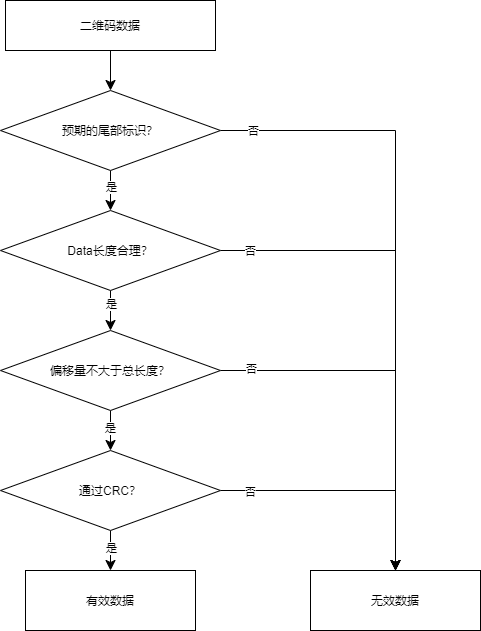
\includegraphics[scale=0.6]{figures/CRC_Check.png}
\caption{数据校验流程}
\end{figure}

\section{本章小结}

本章介绍了一种复杂环境下的高效自适应二维码编解码方法,在已有研究的基础上对部分算法进行加工、合并,针对本项目对已有的技术做出了针对性的改进。创新性的提出了二维码的位置缓存解码方案、自适应的高精度格点识别方法、基于逻辑斯蒂回归的色彩分类模型以及基于二维码的数据传输协议,实现了针对这一特殊场景下在速率与可靠性较ISO二维码远高的自定义二维码及其编解码方案。